\documentclass[11pt]{article}
\usepackage[margin=1in]{geometry}
\usepackage{amsmath,amssymb,amsthm,booktabs,graphicx,hyperref,xcolor,tikz}
\usetikzlibrary{arrows.meta,positioning,fit,backgrounds}
\usepackage[numbers]{natbib}
\usepackage{caption}
\newtheorem{theorem}{Theorem}
\newtheorem{proposition}{Proposition}
\newcommand{\todo}[1]{\textcolor{red}{[TODO: #1]}}
\newcommand{\E}{\mathcal{E}}
% RULE: every empirical number below is a macro from generated/numbers.tex or a table/figure in generated/,
% produced by scripts/make_paper1.py, scripts/plot_v3.py, scripts/plot_v6.py from provenance-stamped results/*.json.
% Never type a result by hand. Pre-registrations: papers/latent-hindsight-planning/*_preregistration.md.
% generated by scripts/make_paper1.py -- DO NOT EDIT
% provenance theory_hindsight: commits ['6e7a3ea'], dirty=False, seeds/runs=3
% provenance realdata_hindsight: commits ['0274fa0', '0603271'], dirty=False, seeds/runs=3
% provenance sealed_v3_hybrid: commits ['41de4eb'], dirty=False, seeds/runs=3
% provenance mujoco_v3_main: commits ['9398e5f', 'e554525'], dirty=False, seeds/runs=3
% provenance mujoco_v3_ksweep: commits ['a406392', 'b7d8f7a'], dirty=False, seeds/runs=3
% provenance mujoco_v3_rho: commits ['e554525'], dirty=False, seeds/runs=3
% provenance mujoco_v3_noise2: commits ['3c40ae8'], dirty=False, seeds/runs=3
% provenance identification_v4: commits ['0ec4d38'], dirty=False, seeds/runs=3
% provenance diag_confound: commits ['eb344b9'], dirty=False, seeds/runs=1
% provenance river: commits ['a36ff57'], dirty=False, seeds/runs=3
% provenance river_v2: commits ['e2950d0'], dirty=False, seeds/runs=3
% provenance throw: commits ['55e206d', '72a91db'], dirty=False, seeds/runs=3
% provenance mujoco_v3_delay: commits ['12fca02', '1db147f', 'c1ae4eb'], dirty=False, seeds/runs=12
% provenance hier_main: commits ['484bf30', '5e36910', '789a0d5'], dirty=False, seeds/runs=3
% provenance latency: commits ['5e36910'], dirty=False, seeds/runs=2
\newcommand{\cfDipPin}{0.000}
\newcommand{\cfDipStd}{-0.286}
\newcommand{\cfRPin}{0.996}
\newcommand{\dlCapture}{66.4\%}
\newcommand{\dlGainTwenty}{36.7\%}
\newcommand{\dlGainZero}{2.3\%}
\newcommand{\dlOracleTwenty}{0.447}
\newcommand{\dlOracleZero}{0.975}
\newcommand{\dlPostTwenty}{0.633}
\newcommand{\dlPostVsSgdTwenty}{0.722}
\newcommand{\dlPostVsSgdZero}{0.991}
\newcommand{\dlPostZero}{0.977}
\newcommand{\dlSgdTwenty}{0.876}
\newcommand{\dlSgdZero}{0.986}
\newcommand{\hiCapture}{90.4\%}
\newcommand{\hiDiffBoth}{+0.31}
\newcommand{\hiDiffFresh}{-0.11}
\newcommand{\hiDiffHiBoth}{+0.39}
\newcommand{\hiDiffHiFresh}{-0.01}
\newcommand{\hiDiffHiNone}{+0.00}
\newcommand{\hiDiffHiWind}{+0.28}
\newcommand{\hiDiffLoBoth}{+0.24}
\newcommand{\hiDiffLoFresh}{-0.20}
\newcommand{\hiDiffLoNone}{+0.00}
\newcommand{\hiDiffLoWind}{+0.15}
\newcommand{\hiDiffNone}{+0.00}
\newcommand{\hiDiffWind}{+0.21}
\newcommand{\hiEpisodes}{150}
\newcommand{\hiFlatBoth}{0.04}
\newcommand{\hiFlatFresh}{0.01}
\newcommand{\hiFlatHindBoth}{0.00}
\newcommand{\hiFlatHindFresh}{0.00}
\newcommand{\hiFlatHindNone}{0.00}
\newcommand{\hiFlatHindWind}{0.00}
\newcommand{\hiFlatNone}{0.41}
\newcommand{\hiFlatWind}{0.09}
\newcommand{\hiFwdBoth}{0.55}
\newcommand{\hiFwdFresh}{0.36}
\newcommand{\hiFwdNone}{1.00}
\newcommand{\hiFwdWind}{0.73}
\newcommand{\hiHindBoth}{0.86}
\newcommand{\hiHindFresh}{0.25}
\newcommand{\hiHindNone}{1.00}
\newcommand{\hiHindWind}{0.94}
\newcommand{\hiOracleBoth}{0.89}
\newcommand{\hiOracleFresh}{0.94}
\newcommand{\hiOracleNone}{1.00}
\newcommand{\hiOracleWind}{0.98}
\newcommand{\hiPfBoth}{0.83}
\newcommand{\hiPfFresh}{0.37}
\newcommand{\hiPfNone}{1.00}
\newcommand{\hiPfWind}{0.95}
\newcommand{\hiResidBoth}{0.77}
\newcommand{\hiResidFresh}{0.39}
\newcommand{\hiResidNone}{1.00}
\newcommand{\hiResidWind}{0.95}
\newcommand{\hiSgdBoth}{0.64}
\newcommand{\hiSgdFresh}{0.37}
\newcommand{\hiSgdNone}{1.00}
\newcommand{\hiSgdWind}{0.84}
\newcommand{\idPredDip}{0.138}
\newcommand{\idPredEnd}{0.888}
\newcommand{\idPredTwenty}{0.773}
\newcommand{\idWindTwenty}{0.837}
\newcommand{\ksGainForty}{34.1\%}
\newcommand{\ksGainOne}{0.4\%}
\newcommand{\ksHeadForty}{49.1\%}
\newcommand{\latCPU}{Intel Xeon Processor @ 2.30GHz}
\newcommand{\latFwdFour}{57}
\newcommand{\latFwdOne}{51}
\newcommand{\latObsPost}{0.68}
\newcommand{\latPfFour}{51}
\newcommand{\latPfOne}{57}
\newcommand{\latPostFour}{82}
\newcommand{\latPostOne}{79}
\newcommand{\mjCaptureBoth}{60.7\%}
\newcommand{\mjCaptureWind}{60.5\%}
\newcommand{\mjFreshPost}{1.019}
\newcommand{\mjFreshResid}{1.369}
\newcommand{\mjGainLatent}{0.959}
\newcommand{\mjGainResid}{1.019}
\newcommand{\mjLatentBoth}{0.768}
\newcommand{\mjLatentWind}{0.749}
\newcommand{\mjOracleBoth}{0.691}
\newcommand{\mjOracleWind}{0.652}
\newcommand{\mjPostBoth}{0.776}
\newcommand{\mjPostVsSgdBoth}{0.876}
\newcommand{\mjPostVsSgdWind}{0.870}
\newcommand{\mjPostWind}{0.755}
\newcommand{\mjSgdBoth}{0.886}
\newcommand{\mjSgdWind}{0.867}
\newcommand{\nzAdaptOne}{0.840}
\newcommand{\nzAdaptZero}{0.793}
\newcommand{\nzFixedOne}{1.001}
\newcommand{\nzFixedZero}{0.821}
\newcommand{\nzPostOne}{0.803}
\newcommand{\nzPostZero}{0.790}
\newcommand{\nzResidOne}{0.981}
\newcommand{\nzResidZero}{0.783}
\newcommand{\rdHybridFwd}{0.817}
\newcommand{\rdHybridSgd}{1.001}
\newcommand{\rdHybridSigFwd}{44/45}
\newcommand{\rdHybridWorseSgd}{25/45}
\newcommand{\rdOneStep}{0.959}
\newcommand{\rdRecords}{15}
\newcommand{\rdResidTen}{1.628}
\newcommand{\rdSgdFwdTen}{0.817}
\newcommand{\rdSgdOne}{0.892}
\newcommand{\rdTenStep}{0.887}
\newcommand{\rhoOne}{0.736}
\newcommand{\rhoZero}{1.221}
\newcommand{\rvOneFlat}{1.000}
\newcommand{\rvOneFwd}{0.577}
\newcommand{\rvOneHind}{0.363}
\newcommand{\rvThreeFwd}{0.89}
\newcommand{\rvThreeOracle}{0.54}
\newcommand{\rvTwoFwd}{0.333}
\newcommand{\rvTwoHind}{0.333}
\newcommand{\rvTwoOracle}{1.000}
\newcommand{\thForward}{1536}
\newcommand{\thFreshFwd}{1522}
\newcommand{\thFreshHind}{1619}
\newcommand{\thHindsight}{2.3}
\newcommand{\thResidAdd}{0.090}
\newcommand{\thResidual}{13393}
\newcommand{\thSigmaSq}{0.090}
\newcommand{\thSigmaSqD}{0.18}
\newcommand{\thSwitchForget}{670}
\newcommand{\thSwitchFwd}{1525}
\newcommand{\thSwitchHind}{2292}
\newcommand{\thT}{4000}
\newcommand{\thTexcess}{0.18}
\newcommand{\twAttempts}{10}
\newcommand{\twEpisodes}{600}
\newcommand{\twFirstBoth}{9.0\%}
\newcommand{\twFirstDamp}{24.3\%}
\newcommand{\twFirstFresh}{9.0\%}
\newcommand{\twFirstWind}{9.0\%}
\newcommand{\twFwdMissBoth}{0.84}
\newcommand{\twFwdMissDamp}{0.49}
\newcommand{\twFwdMissFresh}{0.84}
\newcommand{\twFwdMissWind}{0.73}
\newcommand{\twHindBoth}{0.238}
\newcommand{\twHindDamp}{0.321}
\newcommand{\twHindFresh}{1.269}
\newcommand{\twHindLastBoth}{0.19}
\newcommand{\twHindLastDamp}{0.15}
\newcommand{\twHindLastFresh}{1.01}
\newcommand{\twHindLastWind}{0.12}
\newcommand{\twHindWind}{0.189}
\newcommand{\twOracleGapBoth}{1.8}
\newcommand{\twOracleGapDamp}{2.2}
\newcommand{\twOracleGapFresh}{9.9}
\newcommand{\twOracleGapWind}{6.0}
\newcommand{\twResidBoth}{0.391}
\newcommand{\twResidDamp}{0.603}
\newcommand{\twResidFresh}{1.407}
\newcommand{\twResidWind}{0.180}


\title{Planning in Hindsight:\\Inferring the Latent Variables a World Model Could Not Predict}
\author{\todo{authors}}
\date{}

\begin{document}
\maketitle

\begin{abstract}
A world model used for planning must predict the consequences of actions, but the world contains factors the model
cannot observe: a weak motor, a crosswind, a slippery floor, a sensor that lags. In the latent-variable formulation of
world models these factors are a latent $z$ that the predictor cannot know in advance. We argue that when $z$
\emph{persists}, the agent should not plan around it but \emph{infer it after the fact}: every executed action produces
an observed outcome, the energy between prediction and outcome is evidence about $z$, and minimising that energy over $z$
before planning the next action turns surprise into knowledge. We call this \emph{hindsight latent-variable planning}.
We show that forward planning, residual reuse and test-time latent inference are one filter at three settings of its
gain; that hindsight is never worse than forward planning and is strictly, logarithmically-versus-linearly better when
$z$ persists; and that it cannot help when $z$ is redrawn. Experiments with learned world models in MuJoCo confirm each
prediction under pre-registered rules. When a thrower faces persistent unknown damping and wind, hindsight reduces the
miss distance to \twHindBoth{} of forward planning by the second attempt onwards, beats residual reuse (\twResidBoth) when
the latent is multiplicative, and loses to forward planning (\twHindFresh) when the latent is redrawn every attempt, as
theory requires. Under observation latency its advantage grows with the delay, reaching \dlPostTwenty{} of forward cost
at 20 steps versus \dlSgdTwenty{} for online fine-tuning. Learned hindsight does not reach the oracle that is given the
true $z$, and in a hierarchical river-crossing task it did not rescue failed subgoals; we report both.
\end{abstract}

% ---------------------------------------------------------------------------------------------------------------
\section{Introduction}

A planning agent with a world model works in two modes. Before acting it predicts; after acting it observes. Most
model-based planners use only the first mode: they roll the predictor forward, optimise an action sequence against a
cost, execute part of it, observe the new state, and plan again from that state with the \emph{same} predictor
\citep{chua2018pets,hjepa_2610_06805}. The observation is used as a new starting point, not as evidence about why the
previous prediction was wrong.

This matters because world models are deployed in worlds they were not trained on. In the latent-variable view of
world models \citep{lecun2022path}, the predictor takes a latent $z$ that accounts for what the state and action do not
determine. During planning $z$ is unknown, and the standard options are to fix it at a nominal value, to sample it, or to
plan against the worst case. All three treat $z$ as \emph{unpredictable}. But many of the factors that defeat plans in
practice are not unpredictable: they are \emph{unknown and persistent}. A robot's gripper slips the same way on every
grasp of the same object. A drone faces the same crosswind for minutes. The motor that was weak on the first step is weak
on the hundredth. For such factors, every executed action is an experiment, and the outcome is information that a planner
that only predicts throws away.

\paragraph{The idea.} Hindsight latent-variable planning keeps the predictor frozen and moves the adaptation into $z$.
After each executed segment, the agent computes the energy between what it predicted and what happened, infers the
posterior over $z$ that makes the past observations least surprising, and plans the next segment under that posterior
(Figure~\ref{fig:arch}). Nothing about the predictor changes; what changes is the agent's belief about the world it is
in. This is the planning counterpart of a familiar principle: a forecaster who missed yesterday should not just restart
from today's weather, but ask what it got wrong.

\paragraph{Why this matters for hierarchical planning.} Hierarchical planners
\citep{lecun2022path,hjepa_2610_06805} decompose a long task into subgoals. A persistent, unmodelled $z$ biases every
level the same way: if the high level proposes a subgoal that is infeasible under the true $z$, the low level fails, the
high level replans from the new state with the same model, and proposes the same kind of subgoal again. Retrying does
not help, because the failure is a property of the world, not of chance. Hindsight inference is the mechanism that
lets the high level learn from a subgoal failure. We state this as a theorem (Theorem~\ref{thm:hier}) with two
conditions, persistence and detection before irreversibility, and we report that our hierarchical experiments did
\emph{not} meet them (Section~\ref{sec:hier}).

\paragraph{Contributions.}
\begin{enumerate}
\item \textbf{A formulation.} Hindsight planning as inference over the latent variable of an energy-based world model,
followed by planning under the posterior (Section~\ref{sec:method}). Forward planning, residual reuse
\citep{cwm_2611_24778} and test-time latent inference \citep{t2z_2610_22364} are the same filter at gain $0$, gain $1$ and
the Bayes-optimal gain.
\item \textbf{When it works, provably.} Five results (Section~\ref{sec:theory-summary}, Appendix~\ref{sec:theory}):
hindsight is never worse; it has $O(\sigma^2 d\log T)$ regret against $\Theta(T)$ for forward planning when $z$ persists;
it gains nothing when $z$ is fresh; residual reuse is inconsistent; and a hierarchical planner benefits only if the
surprise is detected before failure is irreversible.
\item \textbf{When it works, measurably.} Pre-registered experiments with learned ensemble world models that separate the
three conditions the theory names: persistence (fresh-draw controls and an AR(1) persistence sweep), commitment
(open-loop chunk length, one-shot throws) and delayed feedback (observation latency). The gains appear exactly where
the conditions hold and vanish where they do not (Section~\ref{sec:exp}).
\item \textbf{What the inferred latent represents.} Probing the posterior shows that it identifies the predictive
combination of latent factors, not each factor separately; claims about interpretable latents must be made about
identifiable quantities (Section~\ref{sec:probe}).
\end{enumerate}

\begin{figure}[t]\centering
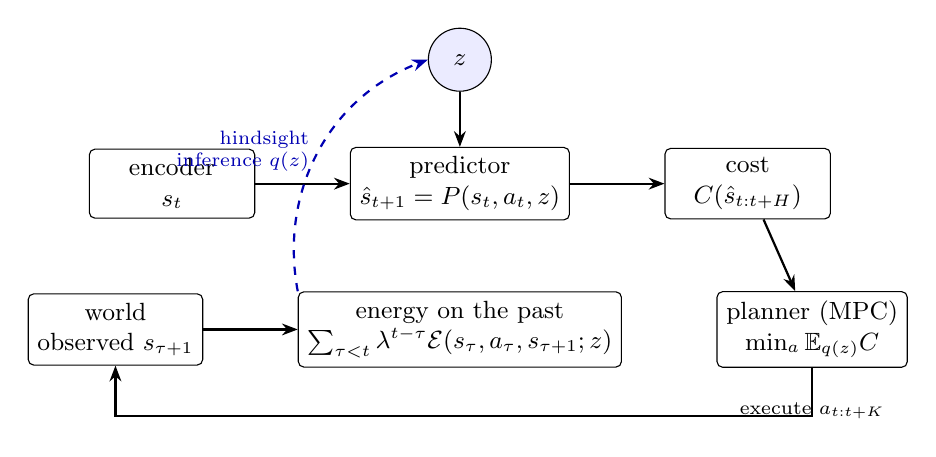
\begin{tikzpicture}[
  box/.style={draw, rounded corners=2pt, minimum height=0.85cm, minimum width=2.1cm, align=center, font=\small},
  lat/.style={draw, circle, minimum size=0.8cm, font=\small, fill=blue!8},
  arr/.style={-{Stealth[length=2mm]}, thick},
  darr/.style={-{Stealth[length=2mm]}, thick, dashed, blue!70!black}]
  \node[box] (enc) {encoder\\$s_t$};
  \node[box, right=1.2cm of enc] (pred) {predictor\\$\hat s_{t+1}=P(s_t,a_t,z)$};
  \node[box, right=1.2cm of pred] (cost) {cost\\$C(\hat s_{t:t+H})$};
  \node[lat, above=0.7cm of pred] (z) {$z$};
  \node[box, below=0.9cm of pred] (energy) {energy on the past\\$\sum_{\tau<t}\lambda^{t-\tau}\E(s_\tau,a_\tau,s_{\tau+1};z)$};
  \node[box, left=1.2cm of energy] (world) {world\\observed $s_{\tau+1}$};
  \node[box, right=1.2cm of energy] (actor) {planner (MPC)\\$\min_a \mathbb E_{q(z)}C$};
  \draw[arr] (enc) -- (pred); \draw[arr] (pred) -- (cost); \draw[arr] (z) -- (pred);
  \draw[arr] (world) -- (energy);
  \draw[darr] (energy.north west) to[bend left=40] node[left, font=\scriptsize, align=right]{hindsight\\inference $q(z)$} (z.west);
  \draw[arr] (cost) -- (actor); \draw[arr] (actor) -- node[below, font=\scriptsize]{execute $a_{t:t+K}$} ++(0,-1.1) -| (world);
\end{tikzpicture}
\caption{Hindsight latent-variable planning. A frozen predictor takes a latent $z$ for the factors it cannot observe.
Forward planning fixes $z$ at its prior. Hindsight planning infers $q(z)$ by minimising the energy between past
predictions and past observations (dashed), then plans under it. Executing a chunk of $K$ actions produces new
observations and closes the loop.}
\label{fig:arch}
\end{figure}

% ---------------------------------------------------------------------------------------------------------------
\section{Hindsight latent-variable planning}
\label{sec:method}

\paragraph{World model.} A predictor $P$ maps a state, an action and a latent to the next state,
$\hat s_{t+1}=P(s_t,a_t,z)$, and defines the energy of an observed transition
\begin{equation}
\E(s_t,a_t,s_{t+1};z)=\tfrac12\big\|s_{t+1}-P(s_t,a_t,z)\big\|^2_{\Sigma^{-1}},
\end{equation}
with $\Sigma$ the predictor's residual covariance. Low energy means the transition is compatible with $z$. In our
experiments $P$ is an ensemble of MLPs trained on simulated transitions in which $z$ is varied; Section~\ref{sec:lim}
discusses what changes when $z$ must be learned without labels.

\paragraph{Hindsight inference.} At time $t$ the agent has a history $\mathcal H_t=\{(s_\tau,a_\tau,s_{\tau+1})\}_{\tau<t}$.
The hindsight posterior is the Gibbs distribution of the accumulated energy,
\begin{equation}
q_t(z)\;\propto\;p(z)\exp\Big(-\sum_{\tau<t}\lambda^{\,t-1-\tau}\,\E(s_\tau,a_\tau,s_{\tau+1};z)\Big),
\label{eq:post}
\end{equation}
where $\lambda\le1$ forgets old evidence so the agent can follow a $z$ that drifts. We use three inference engines:
gradient descent on~\eqref{eq:post} for a point estimate (as in test-time latent optimisation \citep{t2z_2610_22364});
a particle approximation with resampling and an online estimate of the residual variance; and, when $P$ is linear in
$(\theta,w)$ around the nominal model, the exact Gaussian posterior (recursive least squares with forgetting).

\paragraph{Planning under the posterior.} The planner minimises expected cost over action sequences,
\begin{equation}
a^\star_{t:t+H}=\arg\min_{a_{t:t+H}}\;\mathbb E_{z\sim q_t}\Big[\textstyle\sum_{k}C\big(\hat s_{t+k}(a,z)\big)\Big],
\end{equation}
by the cross-entropy method, executes the first $K$ actions open-loop, observes, updates $q$, and replans. The
\emph{forward} planner is the same with $q_t=p$ (or $z$ fixed at the prior mean); the \emph{oracle} is the same with
$q_t=\delta_{z^\star}$.

\paragraph{One filter, three gains.} If $z$ enters additively and follows a random walk of per-step variance $\eta$, the
posterior mean is a Kalman filter on the residual $r_t=s_{t+1}-P(s_t,a_t,\bar z)$ with gain $g_t\in[0,1]$. Forward
planning is $g=0$. Reusing the last residual \citep{cwm_2611_24778} is $g=1$, the right gain only when $\eta\to\infty$.
For persistent $z$ ($\eta=0$) the Bayes gain is $g_t\approx1/t$: average all the evidence. The theory below makes the
consequences of choosing the wrong gain precise.

\paragraph{Hindsight in a hierarchy.} In a hierarchical planner the same $q_t(z)$ is shared by every level. The high
level scores subgoals with $\mathbb E_{q_t}$, so a subgoal that failed because of $z$ becomes \emph{less likely to be
proposed again}, and a subgoal whose feasibility under $q_t$ falls below a threshold is abandoned before the low level
reaches an irreversible state. Theorem~\ref{thm:hier} gives the conditions under which this helps.

% ---------------------------------------------------------------------------------------------------------------
\section{When does hindsight help? Theory}
\label{sec:theory-summary}

Full statements and proofs are in Appendix~\ref{sec:theory}; here is the summary. Let $z=(\theta,w)$ contain a
multiplicative part $\theta$ (it scales the effect of the action) and an additive part $w$, with $d=2$ parameters and
observation noise $\sigma^2$.

\begin{enumerate}
\item \textbf{Dominance} (Theorem~\ref{thm:dominance}). The Bayes hindsight planner is never worse than any forward
planner: a forward plan is always available to it. This is Blackwell's comparison of experiments
\citep{blackwell1953}.
\item \textbf{Persistence is necessary} (Theorem~\ref{thm:fresh}). If $z$ is redrawn at every step, the posterior
predictive equals the prior and hindsight gains nothing. A hindsight planner that assumes persistence is then
misspecified and can be worse.
\item \textbf{Persistence is sufficient for a large gain} (Theorem~\ref{thm:separation}). If $z$ persists, forward
planning pays a constant excess per step, $R_F(T)=\Theta(T)$, while hindsight's regret is $O(\sigma^2 d\log T)$, and its
per-step excess decays as $\sigma^2 d/t$.
\item \textbf{Residual reuse is not hindsight} (Theorem~\ref{thm:residual}). Gain $1$ pays $\sigma^2$ per step forever
under a pure additive $z$, is unstable when $\theta>2\bar\theta$, and is worse than forward planning when there is no
disturbance at all.
\item \textbf{Hierarchy} (Theorem~\ref{thm:hier}). Under persistent $z$, a hierarchical planner whose subgoal choice
ignores outcomes fails with the same probability on every retry. Hindsight's advantage equals the probability that the
subgoal is infeasible \emph{and} the surprise is identified before the failure becomes irreversible.
\end{enumerate}
The theory predicts where the empirical gain should be large: $z$ persistent, actions committed before feedback arrives
(so that a biased model cannot be corrected by fast replanning alone), and enough excitation to identify $z$.

% ---------------------------------------------------------------------------------------------------------------
\section{Experiments}
\label{sec:exp}

\paragraph{Protocol.} Every experiment was pre-registered: hypotheses, decision rules, seeds and the analysis script were
committed before the run, and every failed prediction is reported. Results are written with the git commit and a
clean-tree flag; every number in this paper is generated from those files. Each benchmark has an \emph{oracle gate}: the
planner given the true $z$ must beat forward planning, or the benchmark is not measuring the effect of $z$. Intervals are
95\% paired bootstrap intervals over episodes.

\paragraph{Questions.} (Q1) Does hindsight planning beat forward planning when $z$ persists, with learned models? (Q2)
Is the gain caused by persistence, commitment and delayed feedback, as the theory says, or by something else? (Q3) Does
hindsight inference beat the cheaper alternatives, residual reuse and online fine-tuning? (Q4) What does the inferred
latent represent? (Q5) Does hindsight rescue hierarchical planning?

\subsection{Environments and baselines}
\textbf{Throw-and-retry.} A 1\,kg puck in MuJoCo \citep{todorov2012mujoco} is launched with a chosen initial velocity
$v_0\in[-4,4]^2$\,m/s and flies for 2\,s; the hidden $z$ is the damping ($U[0.5,2]$) and a constant wind force
($\mathcal N(0,0.5^2)$\,N per axis). Each episode has \twAttempts{} throws at random targets under the same $z$; every
throw is a one-shot open-loop decision. Regimes: wind only, damping only, both, and a \emph{fresh} control in which $z$
is redrawn every throw. \twEpisodes{} episodes (3 seeds $\times$ 200).
\textbf{Puck navigation.} The puck is driven by two motors with a hidden actuator gain and a wind force, controlled by
CEM-MPC that executes open-loop chunks of $K$ steps toward a sequence of goals while $z$ and the planner's memory persist.
\textbf{Latency.} The same task with $K=5$ and observations that arrive $d$ steps late; every planner compensates by
rolling its own \emph{believed} model (the predictor under its current belief about $z$) through the actions sent since
the observation, so hindsight improves both the plan and the reconstruction of the present state.

\textbf{Models.} Five-member MLP ensembles trained on 20,000 simulated throws or on random-action trajectories, with $z$
varied during training. The same models are used by every planner. \textbf{Planners.} Forward ($z$ at its prior);
residual reuse \citep{cwm_2611_24778}; online last-layer SGD in the style of test-time model adaptation
\citep{adajepa_2606_32026}; hindsight with the Gaussian posterior, gradient-based latent inference
\citep{t2z_2610_22364}, or particles; and the oracle given the true $z$.

\subsection{Q1: hindsight planning under persistent latents}

\paragraph{Throw-and-retry.} Figure~\ref{fig:v6}a and Table~\ref{tab:throw}. Forward planning misses by the same
distance on every attempt (\twFwdMissBoth\,m in the \emph{both} regime), because nothing it observes changes what it
does. Hindsight learns from the first miss: from the second attempt onwards its miss is \twHindBoth{} of forward's under
both latents, \twHindDamp{} under damping alone and \twHindWind{} under wind alone, all with intervals far below $1$.
This is the empirical form of Theorem~\ref{thm:separation}: a constant per-attempt excess for forward planning, a
decaying one for hindsight.

\begin{table}[t]\centering\small
\begin{tabular}{lcccc}
\toprule
Regime & hindsight & residual reuse & oracle & hindsight / oracle (attempt 10) \\
\midrule
wind & 0.189 [0.180, 0.198] & 0.180 & 0.030 & 6.0$\times$ \\
damping & 0.321 [0.304, 0.338] & 0.603 & 0.138 & 2.2$\times$ \\
both & 0.238 [0.224, 0.252] & 0.391 & 0.125 & 1.8$\times$ \\
fresh & 1.269 [1.255, 1.284] & 1.407 & 0.107 & 9.9$\times$ \\
\bottomrule
\end{tabular}

\caption{Throw-and-retry. Mean miss over attempts 2--\twAttempts{} relative to forward planning (lower is better;
interval: 95\% paired bootstrap). Last column: hindsight's miss on the final attempt divided by the oracle's.}
\label{tab:throw}
\end{table}

\begin{figure}[t]\centering
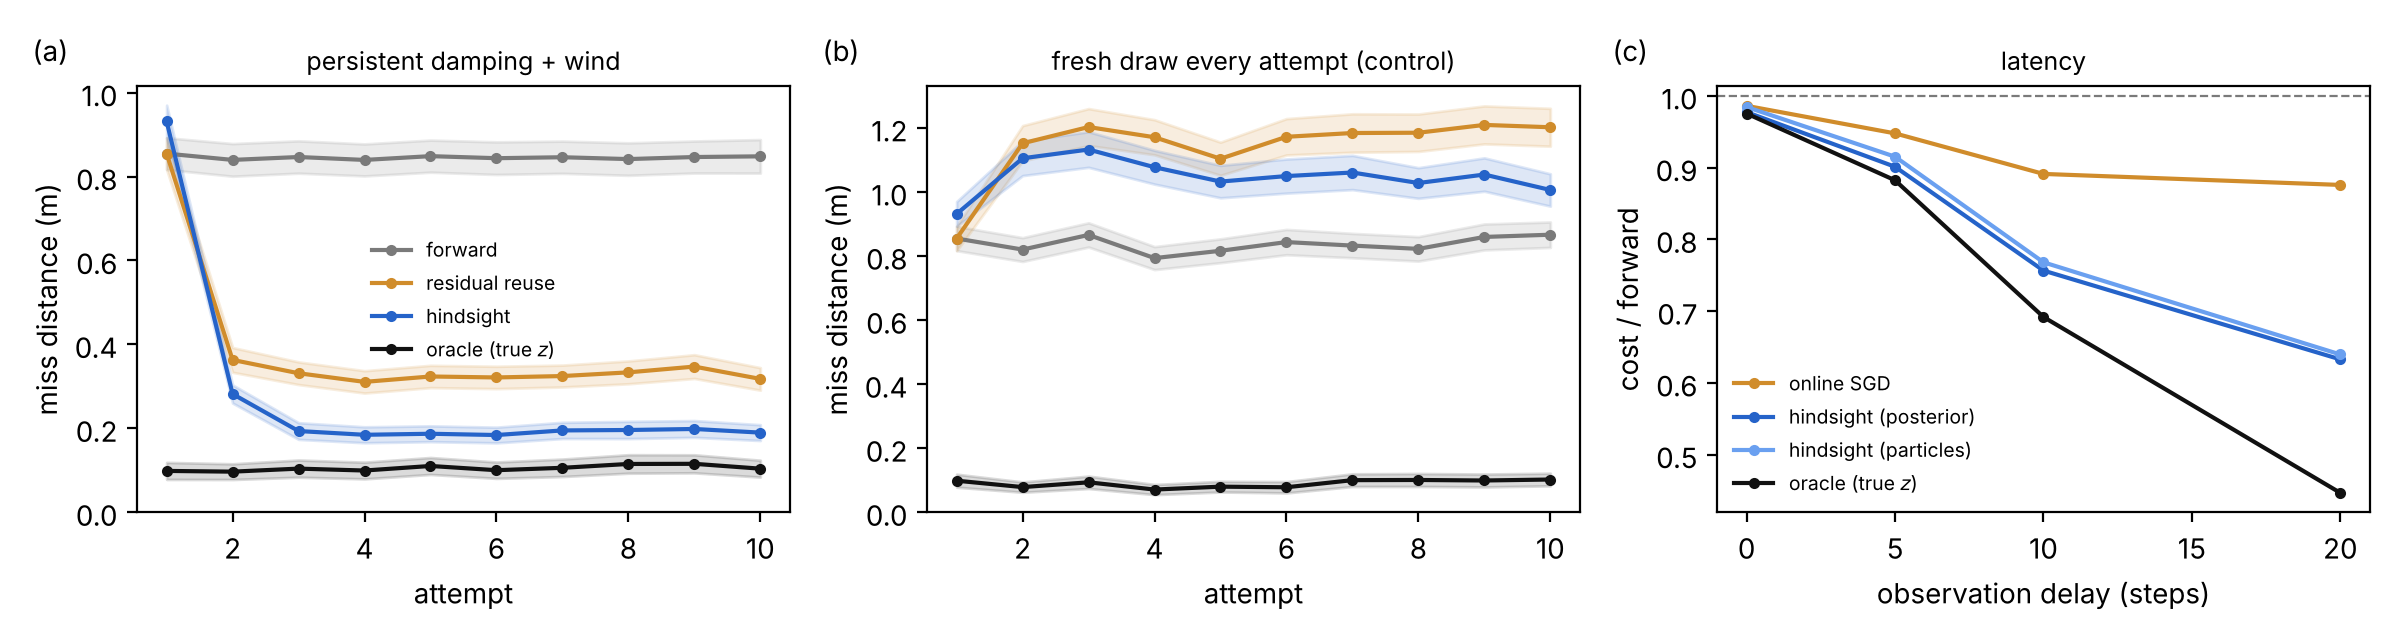
\includegraphics[width=\linewidth]{generated/v6_figure.png}
\caption{(a) Miss distance per attempt under persistent damping and wind; bands are $\pm2$ s.e. (b) The same task with
$z$ redrawn every attempt: hindsight has nothing to learn and is worse than forward planning. (c) Cost relative to
forward planning as observation latency grows.}
\label{fig:v6}
\end{figure}

\paragraph{Puck navigation.} Table~\ref{tab:mujoco}. Under persistent wind with $K=20$, the Gaussian posterior reaches
\mjPostWind{} of forward cost and gradient-based latent inference \mjLatentWind; the oracle reaches \mjOracleWind. The
particle posterior captures \mjCaptureWind{} of the oracle's headroom.

\begin{table}[t]\centering\scriptsize
\begin{tabular}{lccccccc}
\toprule
Regime & posterior & latent (GD) & latent (particles) & hybrid & online SGD & residual reuse & oracle \\
\midrule
wind & 0.755$^{\downarrow}$ & 0.749$^{\downarrow}$ & 0.790$^{\downarrow}$ & 0.751$^{\downarrow}$ & 0.867$^{\downarrow}$ & 0.750$^{\downarrow}$ & 0.652$^{\downarrow}$ \\
both & 0.776$^{\downarrow}$ & 0.768$^{\downarrow}$ & 0.812$^{\downarrow}$ & 0.776$^{\downarrow}$ & 0.886$^{\downarrow}$ & 0.805$^{\downarrow}$ & 0.691$^{\downarrow}$ \\
switching & 0.937$^{\downarrow}$ & 0.865$^{\downarrow}$ & 0.848$^{\downarrow}$ & 0.942$^{\downarrow}$ & 0.976$^{\downarrow}$ & 0.842$^{\downarrow}$ & 0.689$^{\downarrow}$ \\
ood\_gain & 0.964$^{\downarrow}$ & 0.952$^{\downarrow}$ & 0.963$^{\downarrow}$ & 0.966$^{\downarrow}$ & 0.999$^{\downarrow}$ & 1.007$^{\uparrow}$ & 0.945$^{\downarrow}$ \\
gain & 0.979$^{\downarrow}$ & 0.959$^{\downarrow}$ & 0.991 & 0.981$^{\downarrow}$ & 0.997$^{\downarrow}$ & 1.019$^{\uparrow}$ & 0.951$^{\downarrow}$ \\
none & 1.008$^{\uparrow}$ & 0.983$^{\downarrow}$ & 1.012$^{\uparrow}$ & 1.010$^{\uparrow}$ & 0.998$^{\downarrow}$ & 0.994$^{\downarrow}$ & 0.983$^{\downarrow}$ \\
fresh & 1.019$^{\uparrow}$ & 1.000 & 1.287$^{\uparrow}$ & 1.022$^{\uparrow}$ & 0.998$^{\downarrow}$ & 1.369$^{\uparrow}$ & 1.211$^{\uparrow}$ \\
\bottomrule
\end{tabular}

\caption{Puck navigation, $K=20$: cost relative to forward planning. $\downarrow$/$\uparrow$: 95\% interval entirely
below/above 1.}
\label{tab:mujoco}
\end{table}

\subsection{Q2: is the gain caused by persistence, commitment and delayed feedback?}

Each condition of the theory was varied on its own, with everything else fixed.

\paragraph{Persistence.} When $z$ is redrawn at every throw, hindsight is \emph{worse} than forward planning
(\twHindFresh; Figure~\ref{fig:v6}b), as Theorem~\ref{thm:fresh} requires. In puck navigation with AR(1) wind of
persistence $\rho$, the particle posterior's cost ratio falls monotonically from \rhoZero{} at $\rho=0$ to \rhoOne{} at
$\rho=1$ (Table~\ref{tab:rho}). The same method, the same models and the same task go from harmful to strongly helpful as
only the persistence of $z$ changes.

\paragraph{Commitment.} With replanning after every step ($K=1$), hindsight's gain is \ksGainOne{}: fast feedback
absorbs most of the disturbance. With $K=40$ it is \ksGainForty{} against an oracle headroom of \ksHeadForty{}
(Table~\ref{tab:k}). The throw task is the limit of full commitment, and there the gain is largest.

\paragraph{Delayed feedback.} Latency is commitment imposed by the world rather than chosen by the planner.
Pre-registered prediction D1 was that hindsight's gain grows with the delay; it does, from \dlGainZero{} at $d=0$
to \dlGainTwenty{} at $d=20$ (Table~\ref{tab:delay}, Figure~\ref{fig:v6}c). Prediction D2 was that at $d=20$ both
hindsight variants beat forward planning and online fine-tuning; they do (posterior vs online SGD:
\dlPostVsSgdTwenty).

\begin{table}[t]\centering\small
\begin{minipage}{0.48\linewidth}\centering\begin{tabular}{lccccc}
\toprule
$K$ & 1 & 5 & 10 & 20 & 40 \\
\midrule
hindsight gain (wind) & 0.4\% & 0.3\% & 4.3\% & 17.9\% & 34.1\% \\
oracle headroom (wind) & 0.7\% & 1.9\% & 7.7\% & 29.2\% & 49.1\% \\
hindsight gain (both) & 0.8\% & 1.4\% & 5.9\% & 22.6\% & 35.6\% \\
oracle headroom (both) & 1.5\% & 2.5\% & 9.1\% & 35.2\% & 52.0\% \\
\bottomrule
\end{tabular}
\captionof{table}{Gain over forward by
open-loop chunk length $K$.}\label{tab:k}\end{minipage}\hfill
\begin{minipage}{0.48\linewidth}\centering\begin{tabular}{lcccc}
\toprule
$\rho$ & 0.0 & 0.9 & 0.99 & 1.0 \\
\midrule
latent (particles) & 1.221 & 1.058 & 0.840 & 0.736 \\
posterior & 1.018 & 1.015 & 0.819 & 0.707 \\
residual reuse & 1.311 & 0.993 & 0.764 & 0.703 \\
oracle & 1.216 & 0.936 & 0.685 & 0.586 \\
\bottomrule
\end{tabular}
\captionof{table}{Cost relative to forward by
persistence $\rho$ of the wind.}\label{tab:rho}\end{minipage}
\vspace{0.6em}

\begin{tabular}{lcccc}
\toprule
delay (steps) & 0 & 5 & 10 & 20 \\
\midrule
hindsight (posterior) & 0.977 & 0.901 & 0.756 & 0.633 \\
hindsight (particles) & 0.984 & 0.915 & 0.768 & 0.639 \\
online SGD & 0.986 & 0.948 & 0.891 & 0.876 \\
oracle & 0.975 & 0.882 & 0.692 & 0.447 \\
\bottomrule
\end{tabular}

\captionof{table}{Cost relative to forward planning by observation delay (steps), latent \emph{both}, $K=5$.}
\label{tab:delay}
\end{table}

\subsection{Q3: is inference needed, or do cheaper corrections suffice?}

\paragraph{Residual reuse.} Reusing the last residual is the gain-$1$ filter. When $z$ is purely additive it is a
reasonable estimate and ties hindsight on the throw task (\twResidWind{} vs \twHindWind). When $z$ is multiplicative,
the residual of one action says little about the residual of a different action, and hindsight wins: \twHindDamp{} vs
\twResidDamp{} under damping, \twHindBoth{} vs \twResidBoth{} under both. When $z$ is fresh, residual reuse is the worst
planner (\twResidFresh). Under added gust noise in puck navigation it degrades from \nzResidZero{} to \nzResidOne{}
while the Gaussian posterior stays at \nzPostZero{}--\nzPostOne{} (Table~\ref{tab:noise}), as Theorem~\ref{thm:residual}
predicts.

\paragraph{Online fine-tuning.} Updating the predictor's last layer online also uses outcomes, but it spends them on
weights rather than on a low-dimensional latent. It is weaker than the posterior in puck navigation (\mjSgdWind{} vs
\mjPostWind{} under wind) and its advantage barely grows with latency (\dlSgdZero{} at $d=0$, \dlSgdTwenty{} at $d=20$).

\paragraph{Calibration matters.} A particle posterior whose likelihood width is fixed from training residuals chases
deployment noise and loses its gain (\nzFixedZero{} $\to$ \nzFixedOne); estimating the residual variance online restores
it (\nzAdaptZero{} $\to$ \nzAdaptOne). The energy in~\eqref{eq:post} must be scaled to the deployment world, not to
the training set.

\begin{table}[t]\centering\scriptsize
\begin{tabular}{lcccc}
\toprule
gust sd (N) & 0.0 & 0.25 & 0.5 & 1.0 \\
\midrule
posterior & 0.790 & 0.792 & 0.794 & 0.803 \\
latent, adaptive likelihood & 0.793 & 0.797 & 0.810 & 0.840 \\
latent, fixed likelihood & 0.821 & 0.865 & 0.912 & 1.001 \\
residual reuse & 0.783 & 0.795 & 0.833 & 0.981 \\
oracle & 0.708 & 0.710 & 0.712 & 0.716 \\
\bottomrule
\end{tabular}

\caption{Puck navigation under persistent wind plus i.i.d.\ gusts: cost relative to forward planning.}
\label{tab:noise}
\end{table}

\paragraph{Real measured systems.} Five system-identification benchmarks \citep{nonlinear_benchmarks} with official
train/test splits give a test of hindsight \emph{prediction} on data no simulator produced (inputs are logged, so no
planner acts). Over \rdRecords{} test records the Gaussian posterior reduces ten-step prediction error to \rdTenStep{} of
the frozen model's, while residual reuse increases it to \rdResidTen. Online fine-tuning is stronger here
(\rdSgdFwdTen{} at ten steps), and adding the posterior on top of it gives no further gain (\rdHybridSgd), consistent
with residuals that are close to fresh once the model has adapted.

\subsection{Q4: what does the inferred latent represent?}
\label{sec:probe}\label{sec:ident}
A linear probe from the hindsight posterior to the true latent explains \idWindTwenty{} of the wind's variance after 20
transitions, but the actuator gain is poorly identified, and the inferred parameters drop at every chunk boundary. The
reason is identifiability, not failure: the data constrain $\theta a+w$, not $\theta$ and $w$ separately, and each new
action rotates that ridge. Pinning the gain removes the drop (\cfDipStd{} $\to$ \cfDipPin), and the identifiable quantity,
the predicted effect of the next action, \emph{improves} at boundaries and reaches $R^2=$\idPredEnd. Interpretability
claims about inferred latents should be made about identifiable combinations; a probe on an unidentifiable coordinate
measures the excitation of the data, not the quality of the model.

\subsection{Q5: hierarchical planning}
\label{sec:hier}
We built a river-crossing task in which a hierarchical planner chooses between fording (cheap, infeasible under a
strong current) and a bridge (expensive, always feasible), with the current hidden. Across three pre-registered designs
hindsight did not improve success: an abort-and-retreat rule made it worse (\rvOneHind{} vs \rvOneFwd{} for forward), a
fixed plan library had no safe plan once the current was identified (\rvTwoHind{} vs \rvTwoFwd; oracle \rvTwoOracle), and
with per-step MPC the forward planner pushed through (\rvThreeFwd) while the oracle's bridge execution succeeded only
\rvThreeOracle{} of the time, so the main run was not executed. In every design the current was identified within a few steps;
execution and fast feedback decided the outcome. These tasks did not satisfy the second condition of
Theorem~\ref{thm:hier} in a way that a better subgoal choice could exploit. The hierarchical claim remains a theorem
with stated conditions, not an empirical result.

% ---------------------------------------------------------------------------------------------------------------
\section{Limitations}
\label{sec:lim}
\textbf{Not at the oracle.} Pre-registered prediction T4, that hindsight's final throw comes within $2\times$ of the
oracle, failed: the ratio is \twOracleGapBoth{} (both), \twOracleGapDamp{} (damping) and \twOracleGapWind{} (wind). At
20 steps of latency hindsight captures \dlCapture{} of the oracle's improvement. The first throw is also worse than
forward planning (\twFirstBoth{} larger miss under both latents): planning against a broad posterior is more cautious than planning
against its mean. \textbf{Privileged training.} Our predictors are trained with the true $z$ as an input, so the latent
space is given, not learned. In a self-supervised world model \citep{lecun2022path,hjepa_2610_06805} $z$ would have to be
discovered, and its identifiability (Section~\ref{sec:probe}) becomes the central question. \textbf{Scale.}
Low-dimensional state, small MLP ensembles, one simulator and five real benchmarks with logged inputs; no pixels and no
physical robot. \textbf{Excitation.} Multiplicative latents are identified only through variation in the actions;
none of our planners explores deliberately.

\section{Related work}
Latent-variable and energy-based world models and hierarchical planning \citep{lecun2022path,hjepa_2610_06805};
test-time adaptation of world models by latent optimisation \citep{t2z_2610_22364} or weight updates
\citep{adajepa_2606_32026,jepattt_2610_00722}; residual reuse in counterfactual world models \citep{cwm_2611_24778};
hindsight relabeling \citep{andrychowicz2017her}; probabilistic ensembles for MPC \citep{chua2018pets}; adaptive control
and regret \citep{laiwei1982,abbasi2011,simchowitz2020,cassel2020,astrom_wittenmark}; value of information
\citep{blackwell1953}; probing world models \citep{li2023othello,probing_rl_wm_2603_21546}.

\section{Discussion: toward hindsight in hierarchical latent world models}
The results point to a division of labour. The predictor should model what is \emph{the same} across worlds; the
latent should carry what is \emph{constant within} a world; and planning should treat the latent as something to be
inferred from the agent's own history, not marginalised away at every step. In a hierarchical latent world model this
suggests that each level carries its own latent at its own timescale, inferred from the energy of that level's
predictions, and that a high-level subgoal failure is evidence about the high-level latent. Testing this requires three
things our experiments lacked: a latent learned without labels, a hierarchical task in which surprises are identifiable
before they are irreversible, and planners that explore to identify multiplicative latents. We regard these as the next
experiments, not as results.

\bibliographystyle{plainnat}
\bibliography{../refs}

\appendix
% Theory section. All numbers are \input from generated/ (scripts/make_tables.py).
\section{Theory: when is hindsight planning better, and by how much?}
\label{sec:theory}

\paragraph{Setting.} At step $t$ the agent receives a commanded displacement $\delta_t$ (i.i.d., independent of
the past) and chooses a bounded command $|a_t|\le A$. The world responds
\begin{equation}
\Delta s_t=\theta_t a_t+w_t+\varepsilon_t,\qquad \varepsilon_t\sim\mathcal N(0,\sigma^2)\ \text{i.i.d.},
\end{equation}
with cost $c_t=(\Delta s_t-\delta_t)^2$. The hidden disturbance $\phi_t=(\theta_t,w_t)$ has a \emph{gain} part
$\theta_t$ (it scales the command) and an \emph{additive} part $w_t$; its prior is $\mathcal N(m_0,S_0)$ with
$m_0=(\bar\theta,0)$. Let $\mathcal F_t$ be the history $(\delta_{0:t},a_{0:t-1},\Delta s_{0:t-1})$.
A \textbf{forward} planner chooses $a_t$ as a function of $\delta_t$ only (it never conditions on outcomes);
a \textbf{hindsight} planner chooses $a_t$ as a function of $\mathcal F_t$. Regret is measured against the
oracle that knows $\phi_t$ and obeys the same bound; $\varepsilon_t$ is common to all planners and cancels.

\begin{theorem}[Dominance]\label{thm:dominance}
For any prior and any disturbance process, the myopic Bayes hindsight planner
$a^H_t=\arg\min_{|a|\le A}\mathbb E[c_t\mid\mathcal F_t]$, computed under the correct disturbance model,
satisfies $\mathbb E c^H_t\le\mathbb E c^F_t$ for every $t$ and every forward planner $F$.
\end{theorem}
\begin{proof}
$a^F_t$ is a function of $\delta_t$, hence $\mathcal F_t$-measurable, so it is feasible for the minimisation defining
$a^H_t$: $\mathbb E[c^H_t\mid\mathcal F_t]\le\mathbb E[c(a^F_t)\mid\mathcal F_t]$. Because $\delta_t$ is
independent of the past and actions do not move the state that later costs depend on, the law of $c(a^F_t)$
under the hindsight planner's history equals that under $F$'s own history. Take expectations.
This is Blackwell's comparison of experiments~\citep{blackwell1953} specialised to one-step costs.
\end{proof}

\begin{theorem}[No free lunch under fresh disturbances]\label{thm:fresh}
If $\phi_t$ are i.i.d.\ and independent of the past, the posterior predictive of $\phi_t$ given $\mathcal F_t$ equals
the prior, so the correctly specified hindsight planner coincides with the Bayes forward planner and
$\mathbb E c^H_t=\mathbb E c^F_t$. A hindsight planner that \emph{assumes} persistence is misspecified and can be
strictly worse (Table~\ref{tab:theory}, row \emph{fresh}).
\end{theorem}

\begin{theorem}[Linear vs.\ logarithmic regret under persistent disturbances]\label{thm:separation}
Let $\phi_t\equiv\phi\sim\mathcal N(m_0,S_0)$ be persistent and assume targets are reachable
($|\delta_t-w|\le A|\theta|$). Then
\begin{enumerate}
\item the Bayes forward planner pays a constant excess every step,
  $c_F=\sigma_w^2+\sigma_\theta^2\,\mathbb E[\delta^2]/(\bar\theta^2+\sigma_\theta^2)$, so $R_F(T)=c_F\,T$;
\item the certainty-equivalent hindsight planner, and therefore the Bayes hindsight planner, satisfies
\begin{equation}
R_H(T)\le 2\sigma^2\max(1,\kappa)\,d\,\log\!\Big(\tfrac{\lambda_{\max}(V_0)+TL^2/d}{\lambda_{\min}(V_0)}\Big),\quad
V_0=\sigma^2S_0^{-1},\ L^2=A^2+1,\ \kappa=L^2/\lambda_{\min}(V_0),
\end{equation}
with $d=2$; i.e.\ $R_H(T)=O(\sigma^2 d\log T)$, and the per-step excess decays as $\sigma^2 d/t$.
\end{enumerate}
\end{theorem}
\begin{proof}[Proof sketch]
(1) Minimise $\mathbb E[(\theta a+w-\delta)^2]=(\bar\theta^2+\sigma_\theta^2)a^2-2a\bar\theta\delta+\delta^2+\sigma_w^2$
over $a$. (2) With $x_t=(a_t,1)$ and Gaussian conjugacy, the posterior is $\mathcal N(\mu_t,\Sigma_t)$ with
$\Sigma_t=\sigma^2V_t^{-1}$, $V_t=V_0+\sum_{s<t}x_sx_s^\top$. The CE action solves $x_t^\top\mu_t=\delta_t$, so its
error is $x_t^\top(\phi-\mu_t)$ and $\mathbb E[\,\cdot^2\mid\mathcal F_t]=x_t^\top\Sigma_tx_t=\sigma^2\|x_t\|^2_{V_t^{-1}}$.
Since $\|x_t\|^2_{V_t^{-1}}\le\kappa$, we have $u\le\max(1,\kappa)\min(1,u)$, and the elliptical-potential lemma
\citep[Lemma 11]{abbasi2011} gives $\sum_t\min(1,\|x_t\|^2_{V_{t}^{-1}})\le2\log(\det V_T/\det V_0)$; bound
$\det V_T$ by $(\lambda_{\max}(V_0)+TL^2/d)^d$. The Bayes planner is no worse than CE in posterior expectation at
every step because the CE action is feasible for its minimisation.
\end{proof}

\begin{theorem}[Residual reuse is inconsistent for sequential replanning]\label{thm:residual}
Apply the residual-reuse rule of \citet{cwm_2611_24778} at every step: predict
$\Delta s_t(a)=\bar\theta a+r_{t}$ with $r_t=\Delta s_{t-1}-\bar\theta a_{t-1}$, and act on it. Under persistent $\phi$
(unclipped), the error is $e_t=(\theta-\bar\theta)(a_t-a_{t-1})+\varepsilon_t-\varepsilon_{t-1}$. Hence
(i) with a pure additive fault ($\theta=\bar\theta$) it pays excess $\sigma^2$ \emph{every} step, $R(T)=\sigma^2T$,
versus $O(\log T)$ for hindsight; (ii) the commands follow an AR(1) recursion with coefficient
$-(\theta-\bar\theta)/\bar\theta$, which is unstable for $\theta>2\bar\theta$ or $\theta<0$;
(iii) with no disturbance at all it still pays $\sigma^2$ per step while the forward planner pays nothing.
\end{theorem}
\begin{proof}
Substitute $\bar\theta a_t=\delta_t-r_t$ into $e_t=\theta a_t+w+\varepsilon_t-\delta_t$.
\end{proof}
This does not contradict \citet{cwm_2611_24778}: their guarantee is for the counterfactual of \emph{the same event}
(same $\varepsilon$), which is exact under additivity. Item (iii) matches their own report that residual correction
lowers replanning success when there is no disturbance.

\paragraph{Numerical verification.} Table~\ref{tab:theory} checks each statement by Monte-Carlo
(\texttt{wmi/theory.py}, \texttt{scripts/run\_theory.py}).
\begin{table}[h]\centering\scriptsize
\IfFileExists{generated/theory_table.tex}{% generated by scripts/make_tables.py; seeds=[0, 1, 2]; commits=['6e7a3ea']; dirty=False
\begin{tabular}{lccccc}
\toprule
Regime & forward & residual & hindsight\_bayes & hindsight\_forget & $t\cdot$excess (hindsight) \\
\midrule
persistent & 1536.5 $\pm$ 15.2 & 13393.3 $\pm$ 2592.3 & 2.3 $\pm$ 0.0 & 5.3 $\pm$ 0.0 & 0.18 $\pm$ 0.00 \\
persistent\_additive & 1078.0 $\pm$ 11.2 & 360.1 $\pm$ 0.3 & 1.8 $\pm$ 0.0 & 4.8 $\pm$ 0.0 & 0.18 $\pm$ 0.00 \\
persistent\_gain & 543.9 $\pm$ 6.0 & 13444.1 $\pm$ 2613.2 & 1.9 $\pm$ 0.0 & 4.9 $\pm$ 0.0 & 0.18 $\pm$ 0.00 \\
fresh & 1522.4 $\pm$ 0.9 & 4370.6 $\pm$ 1.7 & 1619.1 $\pm$ 1.0 & 1643.1 $\pm$ 1.0 & 1412.80 $\pm$ 1.03 \\
switching & 1525.2 $\pm$ 20.3 & 12916.0 $\pm$ 1456.6 & 2291.7 $\pm$ 104.5 & 669.6 $\pm$ 13.1 & 1845.99 $\pm$ 84.56 \\
none & 76.1 $\pm$ 0.0 & 359.8 $\pm$ 0.3 & 1.5 $\pm$ 0.0 & 4.4 $\pm$ 0.0 & 0.18 $\pm$ 0.00 \\
\midrule
\multicolumn{6}{l}{Closed forms: $c_F T$ = 1551.7; residual (additive) $\sigma^2 T$ = 360.0; $\sigma^2 d$ = 0.18; $T$ = 4000, $M$ = 2000} \\
\bottomrule
\end{tabular}
}{\todo{run scripts/run\_theory.py}}
\caption{Cumulative regret $R(T)$ and $t\cdot\text{excess}_t$ late in the run (constant $\Rightarrow$ $1/t$ decay;
Theorem~\ref{thm:separation} predicts $\sigma^2d$). Mean $\pm$ s.d.\ over seeds.}
\label{tab:theory}
\end{table}

\subsection{Hierarchical planning under persistent surprises}
\label{sec:theory-hier}
A hierarchical planner chooses a route $r\in\{1,\dots,R\}$ (a subgoal sequence) and a low-level controller executes it.
Route $r$ succeeds iff the hidden disturbance lies in its feasible set, $\phi\in\mathcal F_r$; the bridge-like route
$r_0$ is feasible for every $\phi$ but costs more. Executing an infeasible route produces a \emph{surprise} (an observed
transition the nominal model does not predict) after $\tau_{\rm detect}$ steps, and an irreversible failure after
$\tau_{\rm irr}$ steps unless the planner aborts.

\begin{theorem}[Subgoal failure is permanent without hindsight]\label{thm:hier}
Let $\phi$ be persistent. A hierarchical planner whose subgoal choice is a fixed function of the prior (nominal model)
commits to $r^\star$ and re-selects $r^\star$ after every recoverable subgoal failure, so its main-goal failure
probability equals $\Pr(\phi\notin\mathcal F_{r^\star})$ \emph{for any number of retries}. A hierarchical planner whose
subgoal choice conditions on the observed surprise (posterior over $\phi$) and which aborts as soon as
$\Pr(\phi\notin\mathcal F_{r}\mid\text{history})$ exceeds a threshold fails only on the event
$\{\phi\notin\mathcal F_{r^\star}\}\cap\{\tau_{\rm detect}+\tau_{\rm abort}\ge\tau_{\rm irr}\}$.
Hence its advantage is $\Pr\big(\phi\notin\mathcal F_{r^\star},\ \tau_{\rm detect}+\tau_{\rm abort}<\tau_{\rm irr}\big)$,
which is positive iff the surprise is identifiable before the failure becomes irreversible.
If $\phi$ is redrawn independently at every attempt (fresh surprises), retries are independent and the
prior-based planner's failure probability after $n$ retries is $p^{\,n}$; the posterior carries no information about the
next draw, so hindsight gives no advantage (Theorem~\ref{thm:fresh}).
\end{theorem}
\begin{proof}[Proof sketch]
Under persistence the prior-based choice and the low-level outcome are deterministic functions of $\phi$ given the
start state, so every retry reproduces the same failure. The hindsight planner's abort rule triggers on the first
posterior update that makes $r^\star$ infeasible with high probability; it then re-plans over the remaining routes
and $r_0$ is always feasible. Under fresh draws the posterior predictive for the next attempt equals the prior.
\end{proof}
The theorem turns the qualitative claim ``hindsight makes hierarchical planning robust in deployment'' into two
testable conditions: \emph{persistence} of the surprise and \emph{detection before irreversibility}.


\end{document}
